Mole.io utilizza una configurazione di MongoDB in grado di garantire un alto grado di scalabilit� del sistema e, contemporaneamente, un ottimo livello di affidabilit�. La configurazione utilizzata prevede l'uso di due funzionalit� fornite da MongoDB: lo \textit{sharding} ed i \textit{replica-set}.

\subsubsection{Sharding}

Lo sharding � una modalit� di salvataggio dei dati che prevede la possibilit� di suddividerli su diversi server. MongoDB utilizza questa funzionalit� per distribuire grandi \textit{data-set} su un numero variabile di macchine e garantire un alto \textit{throughput} del database.





bilanciare il carico di lavoro di ogni server. 




\subsubsection{Replica Set}


+ server che replicano i dati e 




% come abbiamo shardato
% come, nel sistema finale, verr� fatta la replica per HA

\begin{figure}[h]
\centering
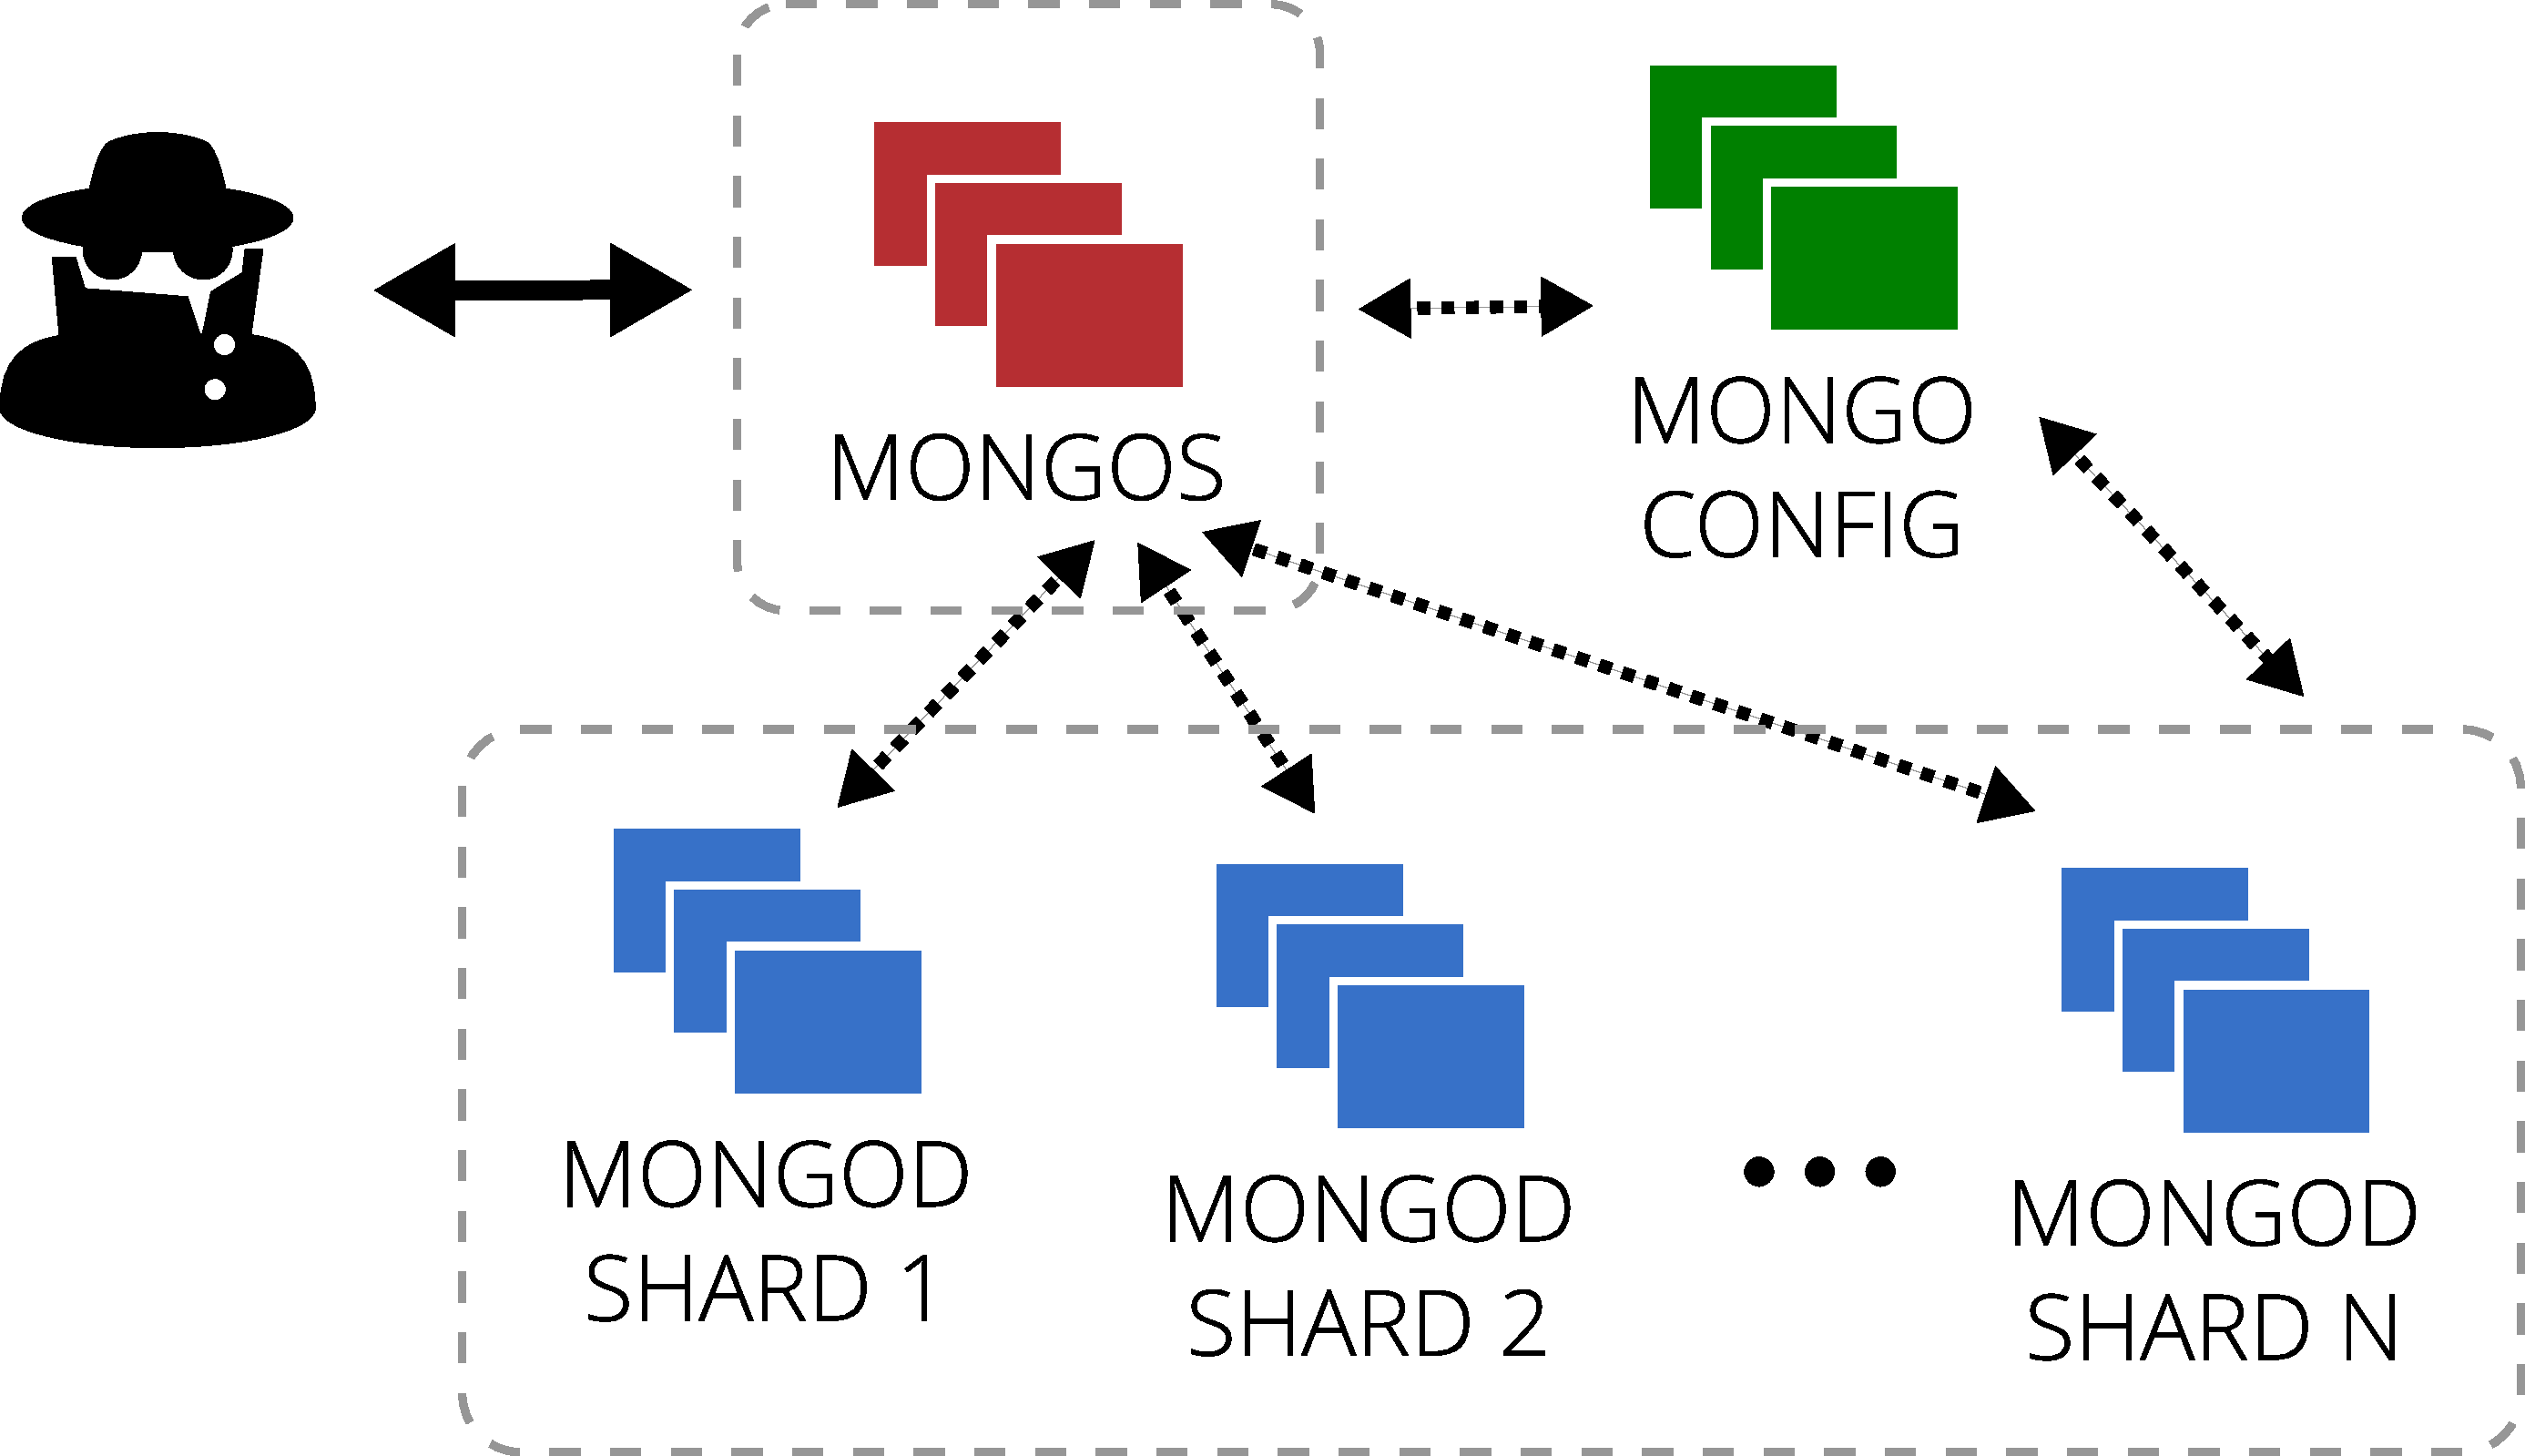
\includegraphics[width=1.0\linewidth]{./img/shard}
\caption[Configurazione di MongoDB per Mole.io]{Configurazione di MongoDB per Mole.io}
\label{fig:shard}
\end{figure}
